\documentclass{beamer}

\usepackage[T2A]{fontenc}
\usepackage[utf8]{inputenc}
\usepackage[russian]{babel}


\hypersetup {
    unicode = true
}

\usetheme{Madrid}
\usecolortheme{whale}

\title[Инструментальная среда]
{Инструментальная среда для анализа программных систем}
\author[А.М. Половцев]{
    А.М. Половцев гр. 63501/13\\
    Руководитель: Ицыксон В.М.\\
    Аттестация №4
}
\date[\today]{}

\begin{document}

\frame{\titlepage}

\begin{frame}
\frametitle{Архитектура инструментального средства}

\begin{figure}[h!]
    \begin{center}
        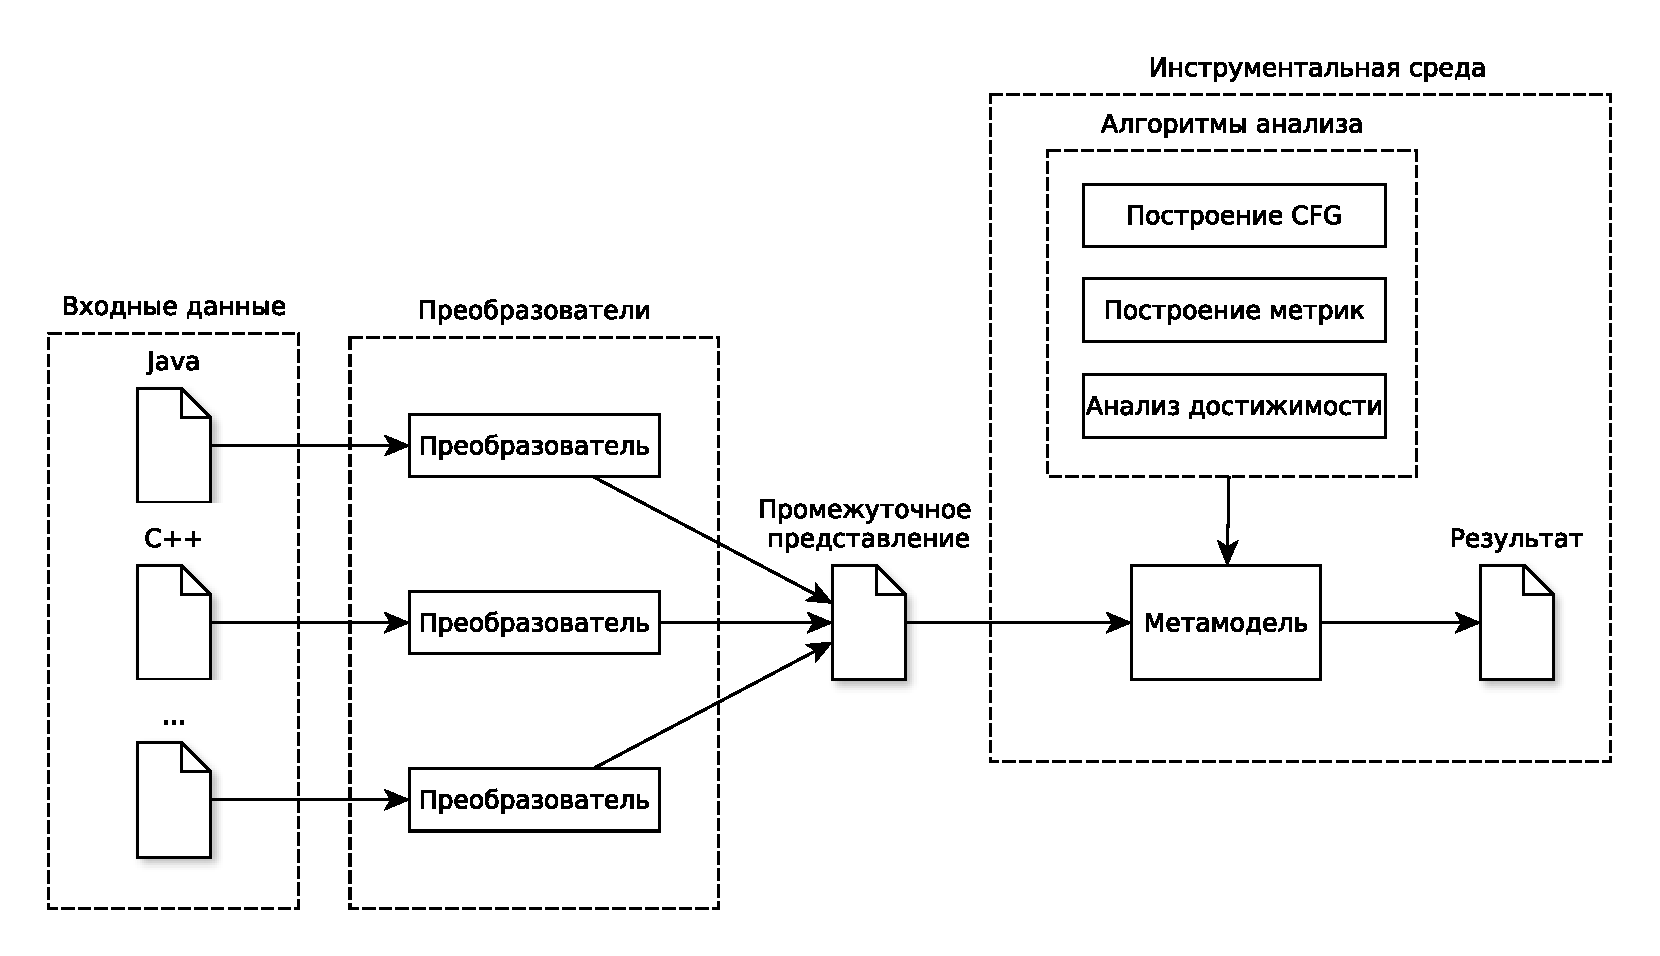
\includegraphics[width=\textwidth]{img/architecture.eps}
    \end{center}
\end{figure}
\end{frame}

\begin{frame}
\frametitle{Что сделано}
    \begin{itemize}
        \item[\checkmark] Парсер Java
        \item[\checkmark] Обратное преобразование из метамодели в программу на языке Java
        \item[\checkmark] Парсер С (частично)
        \item[-] Начата разработка инструментального средства:
            \begin{itemize}
                \item[-] Модульная система для загрузки метамодели
                \item[-] Набор визуализаций (AST, CFG, DDG)
            \end{itemize}
        \item[-] Написание пояснительной записки =)
    \end{itemize}
\end{frame}

\begin{frame}
\frametitle{Спасибо за внимание}
\center{\resizebox{60pt}{80pt}{?}}
\end{frame}

\end{document}
